%%%%%%%%%%%%%%%%%%%%%%%%%%%%%%%%%%%%%%%%%%%%%%%%
% E.Pinault-Bigeard - e.pinault-bigeard@upsti.fr
% http://s2i.pinault-bigeard.com
% CC BY-NC-SA 2.0 FR - http://creativecommons.org/licenses/by-nc-sa/2.0/fr/
%%%%%%%%%%%%%%%%%%%%%%%%%%%%%%%%%%%%%%%%%%%%%%%%
\documentclass[11pt]{article}
%%%%%%%%%%%%%%%%%%%%%%%%%%%%%%%%%%%%%%%%%%%%%%%%
% Package UPSTI_Document
%%%%%%%%%%%%%%%%%%%%%%%%%%%%%%%%%%%%%%%%%%%%%%%%
%%%%%%%%%%%%%%%%%%%%%%%%%%%%%%%%%%%%%%%%%%%%%%%%
% Package UPSTI_Document
%%%%%%%%%%%%%%%%%%%%%%%%%%%%%%%%%%%%%%%%%%%%%%%%
\usepackage{subcaption}
\usepackage[usenames, svgnames, dvipsnames]{xcolor}
\usepackage{UPSTI_Document}
\usepackage{pgfplots}
\usepackage{import}
\definecolor{darkspringgreen}{rgb}{0.09, 0.45, 0.27}

\newcommandx*{\dessinRepereFigGeo}[5][1=\vx{},2=\vy{},3=\vz{},4=,5=0]
	{
		\draw [->,very thick] (0,0) -- (1,0) ;
		\draw [->,very thick] (0,0) -- (0,1) ;
    \fill[white] (0,0) circle (0.13);
    \draw [->,very thick] (0,0) circle (0.13);
    \ifnumequal{#5}{0} {% z vers nous
      \fill[black] (0,0) circle (0.03);
      \draw [->,thick] (0,0) circle (0.04);
    }{% z vers la feuille
  		\begin{scope} [rotate=45]
  			\draw [-,thick] (0,-0.12) -- (0,0.12) ;
  			\draw [-,thick] (-0.12,0) -- (0.12,0) ;
  		\end{scope}
    }
		\draw [anchor=north west] (1.1,0) node {${#1}$};
		\draw [anchor=south west] (0,1.1) node {${#2}$};
		\draw [anchor=north east] (-0.1,0) node {${#3}$};
		\draw [anchor=north west] (-0.1,-0.1) node {${#4}$};
	}

	\usepackage{array}
	\newcolumntype{L}[1]{>{\raggedright\let\newline\\\arraybackslash\hspace{0pt}}m{#1}}
	\newcolumntype{C}[1]{>{\centering\let\newline\\\arraybackslash\hspace{0pt}}m{#1}}
	\newcolumntype{R}[1]{>{\raggedleft\let\newline\\\arraybackslash\hspace{0pt}}m{#1}}

	\usepackage{pifont}% http://ctan.org/pkg/pifont
\newcommand{\cmark}{\color{green}\ding{51}}%
\newcommand{\xmark}{\color{red}\ding{55}}%
\newcommand{\fmark}{\ding{229}}%
\newcommand{\itemc}{\item[\cmark]}%
\newcommand{\itemx}{\item[\xmark]}%
\newcommand{\itemf}{\item[\fmark]}%


\usetikzlibrary[circuits.plc.ladder]            %     
\newlength{\ladderskip}\setlength{\ladderskip}{5\tikzcircuitssizeunit}%5\tikzcircuitssizeunit    = 355pt
\newlength{\ladderrungsep}
\setlength{\ladderrungsep}{.2\ladderskip}
\def\ladderrungend#1{\pgftransformyshift{-#1\ladderskip-\ladderrungsep}}

%---------------------------------%
% Paramètres du package
%---------------------------------%

% Version du document (pour la compilation)
% 1: Document prof
% 2: Document élève
% 3: Document à publier
\newcommand{\UPSTIidVersionDocument}{2}


% Classe
% 1: PTSI				6: PSI*			11: TSI2		16: Spé
% 2: PT	(par défaut)	7: MPSI			12: ATS
% 3: PT*				8: MP			13: PC
% 4: PCSI				9: MP*			14: PC*
% 5: PSI				10: TSI1		15: Sup
%\newcommand{\UPSTIidClasse}{2}



% Matière
% 1: S2I (par défaut)    2: IPT     3: TIPE
% 6: Vie au lycée
\newcommand{\UPSTIvariante}{5}
\newcommand{\UPSTIidMatiere}{0}
\newcommand{\UPSTIintituleMatiere}{Automatique}
\newcommand{\UPSTIsigleMatiere}{Autom}
% Type de document
% 0: Custom*				7: Fiche Métho de			14: Document Réponses
% 1: Cours (par défaut)		8: Fiche Synthèse    		15: Programme de colle
% 2: TD     				9: Formulaire
% 3: TP						10: Memo
% 4: Colle					11: Dossier Technique
% 5: DS						12: Dossier Ressource
% 6: DM						13: Concours Blanc
% * Si on met la valeur 0, il faut décommenter la ligne suivante:
%\newcommand{\UPSTItypeDocument}{Custom}
\newcommand{\UPSTIidTypeDocument}{1}

% Titre dans l'en-tête


% Titre dans l'en-tête

\newcommand{\UPSTIvariante}{5}

\newcommand{\UPSTItitreEnTete}{Automatisme industriel}
%\newcommand{\UPSTItitreEnTetePages}{}
\newcommand{\UPSTIsousTitreEnTete}{Introduction aux API}


% Titre
%\newcommand{\UPSTItitrePreambule}{Automatisme industriel}
\newcommand{\UPSTItitre}{La programmation d'un Automate Industriel}

% Durée de l'activité (pour DS, DM et TP)
\newcommand{\UPSTIduree}{3h30}

% Note de bas de première page
%\newcommand{\UPSTInoteBasDePremierePage}{Geoffrey Vaquette}
% Numéro (ajoute " n°1" après DS ou DM)
\newcommand{\UPSTInumero}{2}

% Numéro chapitre
%\newcommand{\UPSTInumeroChapitre}{1}

% En-tête customisé
%\newcommand{\UPSTIenTetePrincipalCustom}{UPSTIenTetePrincipalCustom}

% Message sous le titre
%\newcommand{\UPSTImessage}{Message sous le titre}


% Référence au programme
%\newcommand{\UPSTIprogramme}{\EPBComp \EPBCompP{B1-02}, \EPBCompP{B2-49}, \EPBCompS{B2-50}, \EPBCompS{B2-51}, \EPBCompP{C1-07}, \EPBCompP{C1-08}}

% Si l'auteur n'est pas l'auteur par défaut
%\renewcommand{\UPSTIauteur}{WWOOOOOOWW}

% Si le document est réalisé au nom de l'équipe
%\newcommand{\UPSTIdocumentCollegial}{1}

% Source
\newcommand{\UPSTIsource}{G. Vaquette, H. Discours}

% Version du document
\newcommand{\UPSTInumeroVersion}{0.2}

%-----------------------------------------------
\UPSTIcompileVars		% "Compile" les variables
%%%%%%%%%%%%%%%%%%%%%%%%%%%%%%%%%%%%%%%%%%%%%%%%


%%%%%%%%%%%%%%%%%%%%%%%%%%%%%%%%%%%%%%%%%%%%%%%%
% Début du document
%%%%%%%%%%%%%%%%%%%%%%%%%%%%%%%%%%%%%%%%%%%%%%%%
\begin{document}
\UPSTIbuildPage

%\UPSTIobjectif{Durant cette activité, nous allons analyser une trame pour l'envoi d'informations sur une étiquette.}

\tableofcontents

\pagebreak

\section{Utilisation de capteurs logiques}
\subsection{Capteur de proximité 3 fils}
On met à votre disposition un capteur de proximité dont les références sont les suivantes :
\UPSTIboiteCentrale{Capteur de proximité}{
	\begin{description}
		\item[Dénomination : ]M12x1, 12-24 VDC PNP 8mmm
		\item[Référence fabricant : ] E2B-M12KN08-WP-B1 2M
		\item[Marque : ] Omron
		\item[Code commande RS : ] 805-2523
	\end{description}
}

\begin{UPSTIactivite}
	\UPSTIquestion{En recherchant sa documentation, câbler ce capteur sur l'entrée 1 de l'automate}
	\UPSTIquestion{Réaliser le programme pour afficher l'état du capteur}
	\begin{center}
		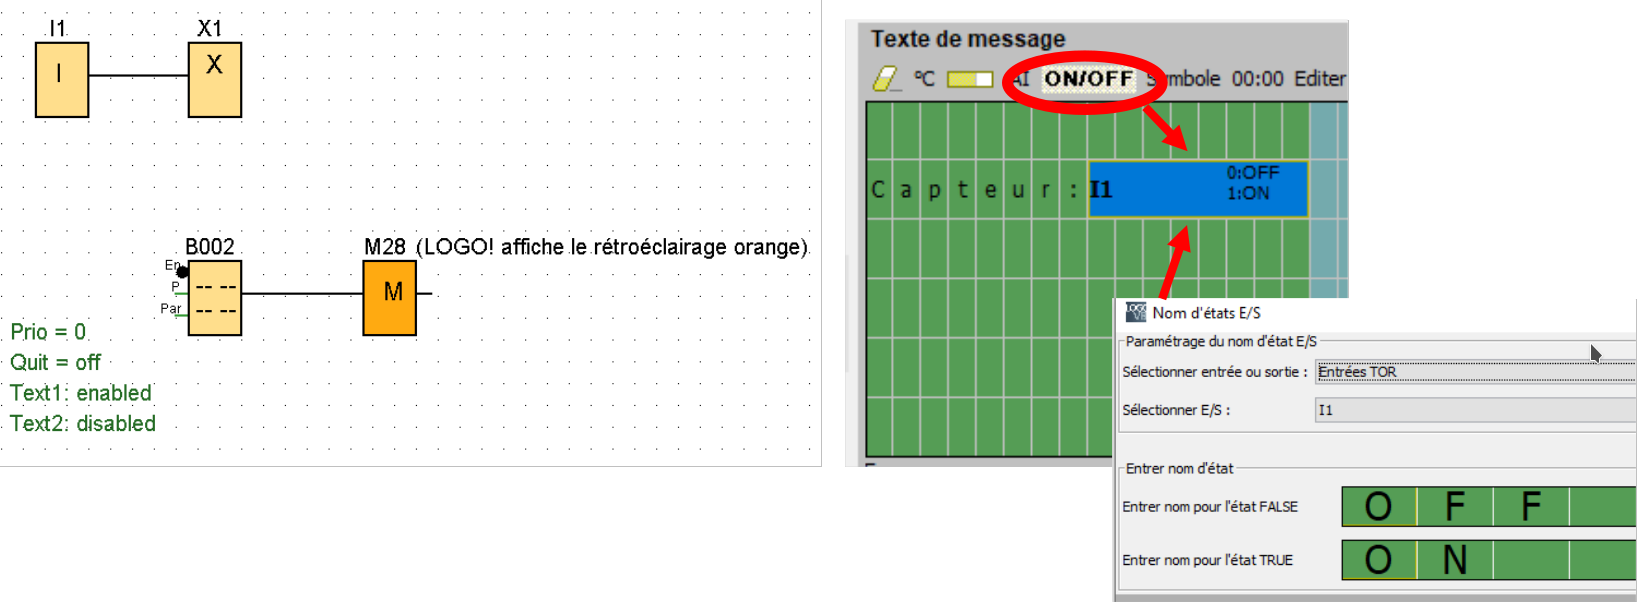
\includegraphics[width=\textwidth]{images/TP04-schemaCaptInductif.png}
	\end{center}
	\UPSTIquestion{Quel type d'objet ce capteur détecte-t-il ? }
	\UPSTIquestion{En effectuant des tests, établir la distance maximale de détection}
\end{UPSTIactivite}

\subsection{Capteur photoélectrique 4 fils}
\UPSTIboiteCentrale{Capteur photoélectrique}{
	\begin{description}
		\item[Dénomination : ]Capteur photoélectrique, Réflexion directe, 450 mm, Cylindrique

		\item[Référence fabricant : ]  GLV18-8-450/115/120
		\item[Marque : ] Pepperl + Fuchs
		\item[Code commande RS : ] 229-034
	\end{description}
}

\begin{UPSTIactivite}
	\UPSTIquestion{En recherchant sa documentation, câbler ce capteur \textbf{en mode Dark On} sur l'entrée 2 de l'automate}
	\UPSTIquestion{Réaliser le programme pour afficher le mot \textbf{Présence} lorsqu'une présence est détectée et \textbf{Absence} sinon.}
	\begin{center}
		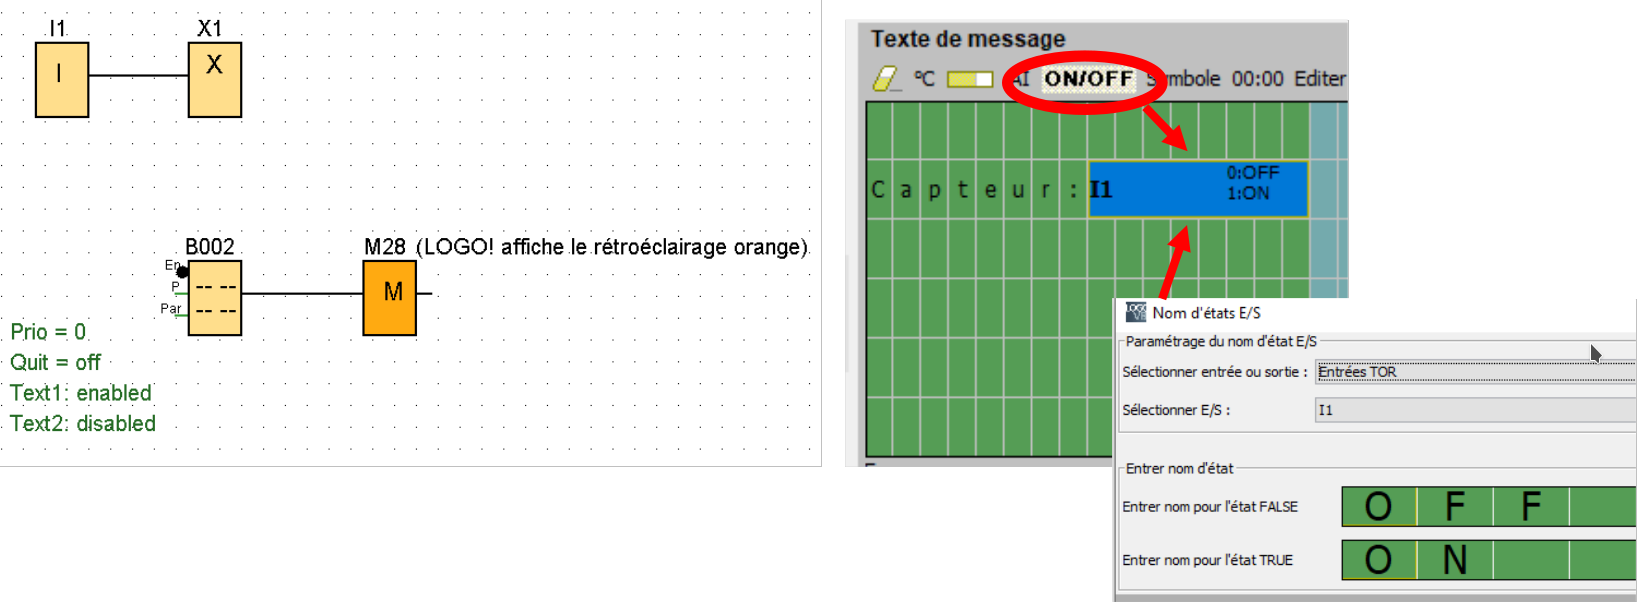
\includegraphics[width=.9\textwidth]{images/TP04-schemaCaptInductif.png}
	\end{center}
	\UPSTIquestion{Quel type d'objet ce capteur détecte-t-il ? }
	\UPSTIquestion{En effectuant des tests, établir la distance maximale de détection pour un objet blanc puis pour un objet noir}
\end{UPSTIactivite}
\pagebreak
\section{Entrées analogiques}
Les entrées I7 et I8 sont utilisable en TOR ainsi qu'en analogique 0-10V. 
Elles sont respectivement identifiée dans le programme par les blocs \textbf{AI1} et \textbf{AI2}. 

\subsection{Cablâge d'un potentiometre}
\begin{UPSTIactivite}
    \UPSTIquestion{Calculer les tensions minimale et maximale du schéma ci-dessous}
    \UPSTIquestion{Expliquer en quoi le schéma suivant n'est pas satisfaisant}
    \begin{center}
        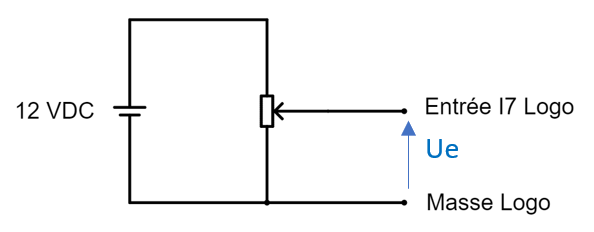
\includegraphics[width=.7\textwidth]{images/TP04-potentiometreDirect.png}
    \end{center}
    \UPSTIquestion{Dessiner un montage respectant la plage de fonctionnement du CAN}
    \vspace{4cm}
    \UPSTIquestion{Réaliser le cablâge}
    \UPSTIquestion{Tester avec le programme suivant :}
    \begin{center}
        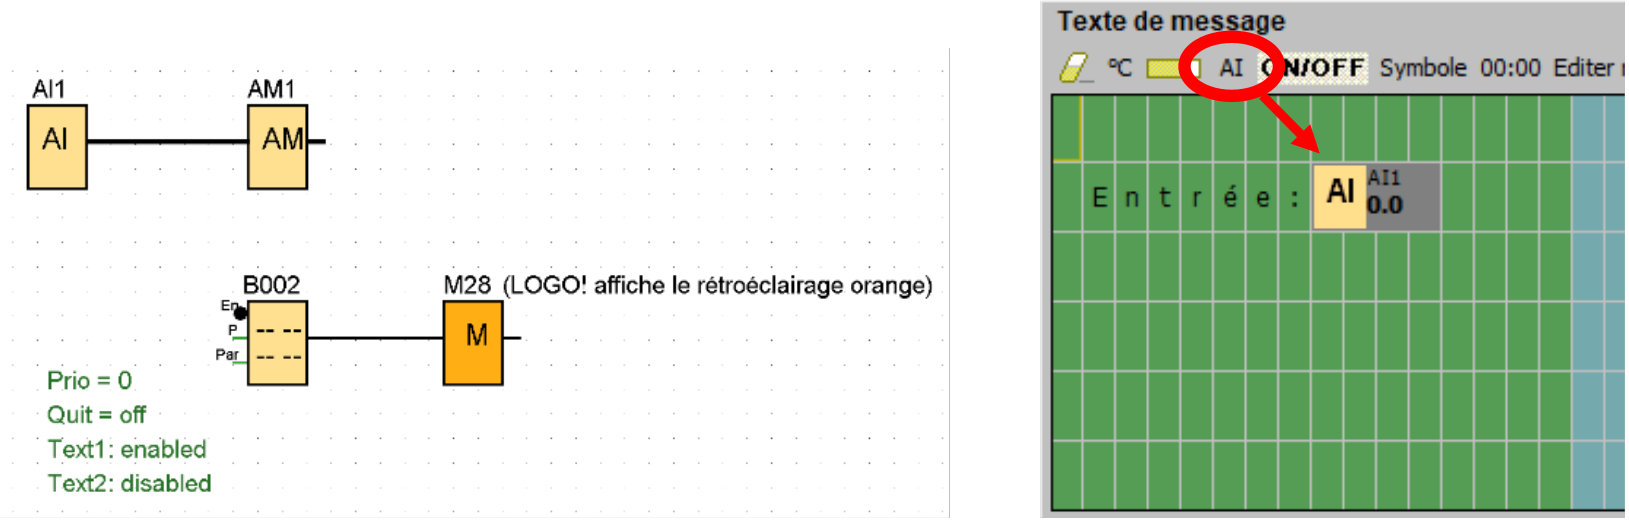
\includegraphics[width=.9\textwidth]{images/TP04-programmePotentiometre.png}
    \end{center}
\end{UPSTIactivite}

\begin{UPSTIactivite}
    \UPSTIquestion{Effectuer les modifications suivantes :}
    \begin{center}
        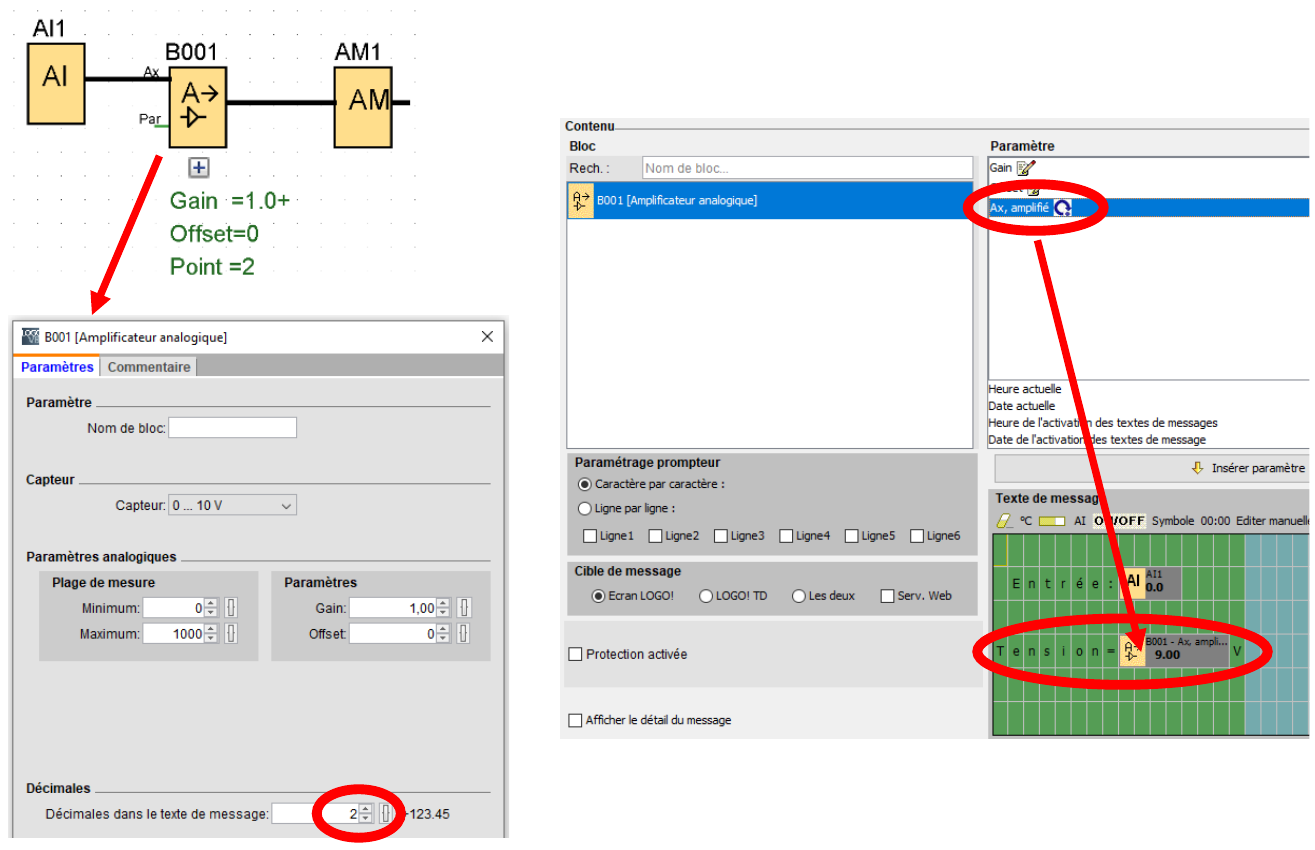
\includegraphics[width=.9\textwidth]{images/TP04-decimales.png}
    \end{center}    
    \UPSTIquestion{Ajouter un bargraph}
    \begin{center}
        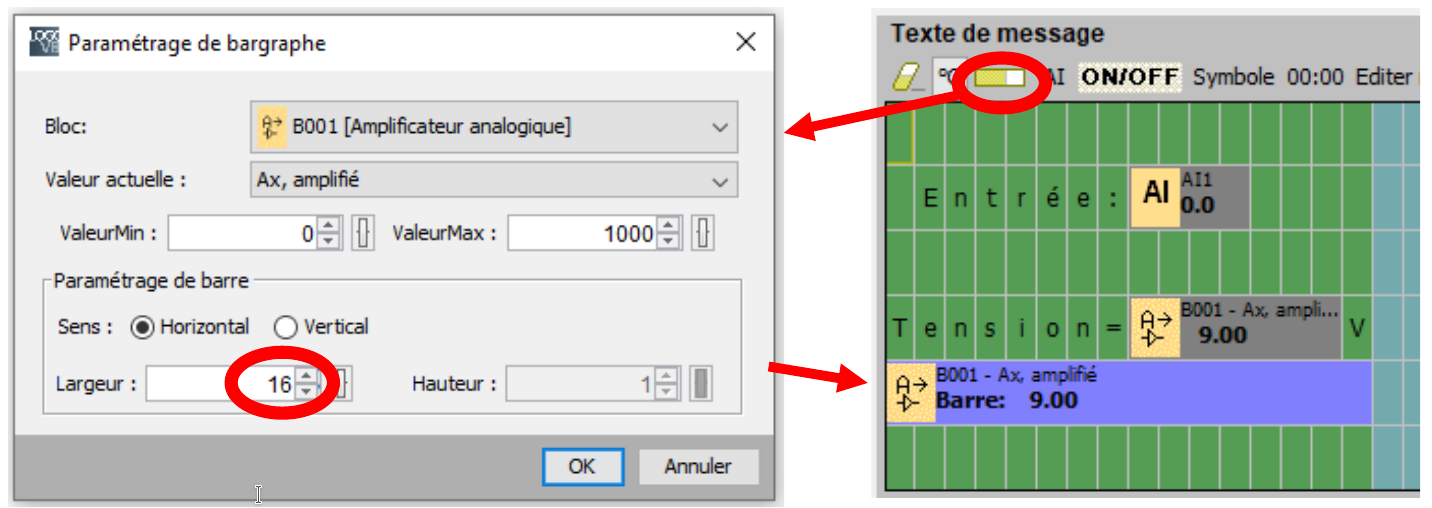
\includegraphics[width=.9\textwidth]{images/TP04-ajoutBarre.png}
    \end{center}    
\end{UPSTIactivite}

\section{Capteur de luminosité}
\UPSTIboiteCentrale{Capteur de luminosité}{
	\begin{description}
		\item[Dénomination : ]TO18 \SI{20}{k\ohm} - \SI{100}{k\ohm}
		\item[Référence fabricant : ] NSL-19M51
		\item[Marque : ] Luna Optoelectronics
		\item[Code commande RS : ] 914-6710
	\end{description}
}

Ce type de capteur de luminosité voit sa résistance varier selon la luminosité qu'il reçoit. 

\begin{UPSTIactivite}
	\UPSTIquestion{Mesurer la résistance du capteur en pleine lumière puis dans le noir}
	On considère le montage suivant : 
	\begin{center}
		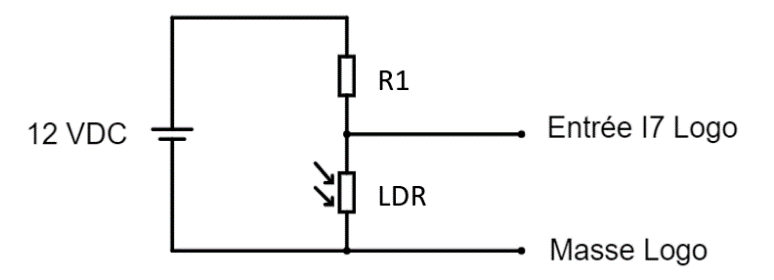
\includegraphics[width=.7\textwidth]{images/TP04-montageLuminosite.png}
	\end{center}
	\UPSTIquestion{Dans quel cas (lumière ou noir), la valeur de la tension aux bornes du capteur sera-t-elle maximale ? }
	\UPSTIquestion{Calculer la valeur de la résistance $R1$ à utiliser pour rester dans la plage de fonctionnement du CAN (0-10V)}
	Au vu de la Caractéristique non linéaire de ce type de capteur (voir Figure~\ref{fig:caracLumi}), nous n'utiliserons ce capteur qu'avec un seuil. 
	\UPSTIquestion{Implémenter le programme suivant et le tester}
	\begin{center}
		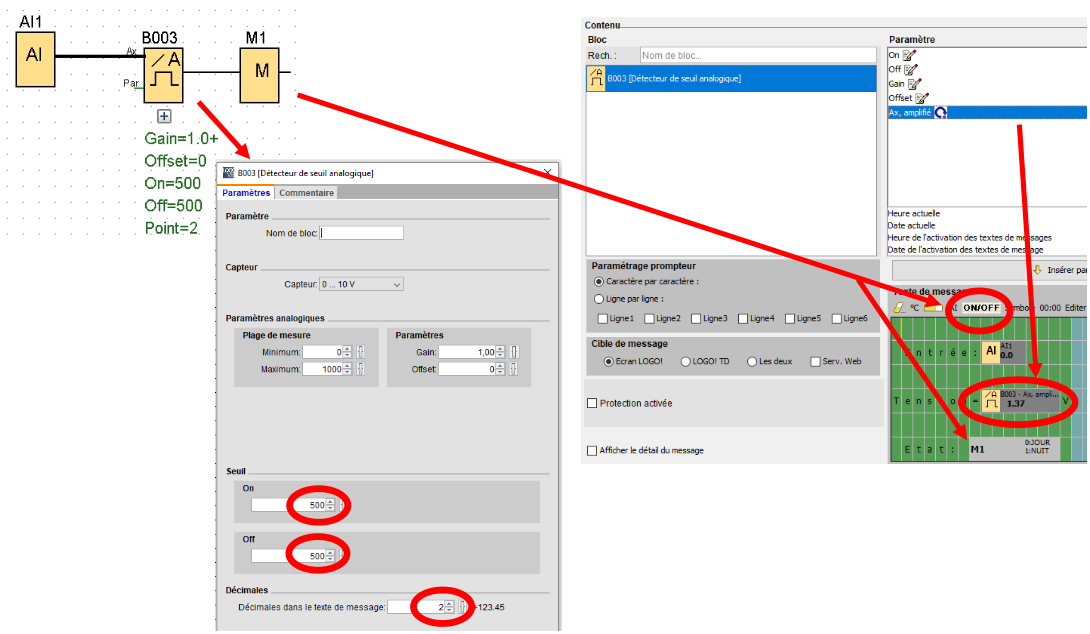
\includegraphics[width=.9\textwidth]{images/TP04-programmeLumi.png}		
	\end{center}
\end{UPSTIactivite}

\begin{figure}
	\centering
	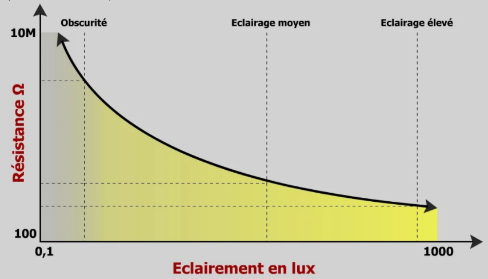
\includegraphics[height=.2\textheight]{images/TP04-caracCapteurLumi.png}
	\caption{Caractéristique typique d'un capteur de luminosité}
	\label{fig:caracLumi}
\end{figure}

\pagebreak
\section{Capteur de température}
\UPSTIboiteCentrale{Capteur de température}{
	\begin{description}
		\item[Dénomination : ]TO92 3 pin \SI{-40}{\deg} - \SI{110}{\deg}
		\item[Référence fabricant : ] LM35CAZ/NOPB
		\item[Marque : ] Texas Instruments
		\item[Code commande RS : ] 533-5878
	\end{description}
}

\begin{UPSTIactivite}
	\UPSTIquestion{A partir de la documentation, calculer la tension de sortie pour une température de \SI{20}{\degree C}
	\UPSTIquestion{En déduire la valeur numérique après conversion par le CAN de l'entrée 7 du Logo}
	}
	\UPSTIquestion{A l'aide de deux blocs de seuils tels qu'utilisés précédemment, écrire un programme qui allume la ventilation au dessus de \SI{26}{\degree C} et le chauffage pour en dessous de \SI{20}{\degree C}}
\end{UPSTIactivite}

\begin{UPSTIactivite}[][Pour aller plus loin]
	\UPSTIquestion{Utiliser la valeur du potentiomettre pour régler les seuils de déclenchement du chauffage et de la ventilation}
\end{UPSTIactivite}
\pagebreak
\section{Capteurs ultasons}
\begin{figure}
	\centering
	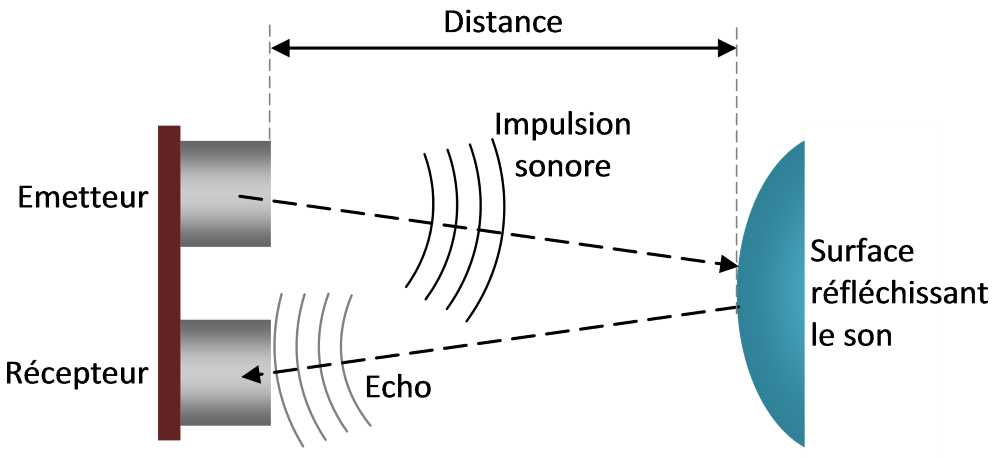
\includegraphics[height=.15\textheight]{images/TP04-ultrasonsPrincipe.jpg}
	\caption{Schéma de principe d'un capteur ultasons}
	\label{fig:ultrasons}
\end{figure}
Un capteur à ultrasons émet à intervalles réguliers de courtes impulsions sonores à haute
fréquence. Ces impulsions se propagent dans l'air à la vitesse du son. Lorsqu'elles rencontrent
un objet, elles se réfléchissent et reviennent sous forme d'écho au capteur.
La mesure du temps entre émission et réception, permet de calculer la distance.

Le modèle étudié, comporte un circuit imprimé avec tous les éléments de calcul de distance.
Ce capteur fournit alors \textbf{un courant} proportionnel à la distance. Ce courant respecte le
format standard 4..20 mA.

\begin{description}
	\item[\SI{0}{cm} : ] \SI{4}{mA}
	\item[\SI{510}{cm} : ] \SI{20}{mA}
\end{description}

\begin{UPSTIactivite}
	\UPSTIquestion{Calculer le coefficient directeur de la droite caractéristique de ce capteur}
	La valeur du courant sera convertie en tension à l'aide d'une résistance. 
	\UPSTIquestion{Dessiner un schéma comportant une alimentation \SI{24}{V} en série avec le capteur ultrason puis une résistance}
	\UPSTIquestion{Calculer la valeur de la résistance pour que la tension maximale soit de \SI{10}{V}}
	\UPSTIquestion{Réaliser le montage et réaliser un programme qui affiche la valeur de l'entrée analogique}
	\UPSTIquestion{Ajouter la valeur du courant puis un bargraph montrant la distance}
	\begin{center}
		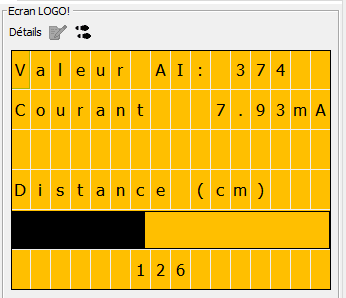
\includegraphics[height=.15\textheight]{images/TP04-attenduUltrason.png}
	\end{center}
	
\end{UPSTIactivite}

\end{document}
